  \subsection{Introduction}
  \begin{definition}
  A \textbf{discrete dynamical system} is a triple $(\NN,X,\Phi)$ with $X$ a non empty set (the state space) and an operation $\Phi : \NN \times X \to X$, so that
  $\Phi(0,x) = x$ and $\Phi(n,\Phi(m,x)) = \Phi(n+m, x)$. 
  Thus, a discrete dynamical system is the model of a system, that evolves over discrete time steps.
  \end{definition}
  The simplest case of a discrete dynamical system, is when the state space is 1-dimensional (say $X \subseteq \RR$) and 
  the transition function only depends on the previous value, i.e. $\Phi(1,x) = f(x)$ for some $f : \RR \to \RR$. 
  Then the dynamical system can be written by the recurrence relation $x_{n+1} = f(x_n)$ with initial condition $x_0 \in \RR$.
  A chaotic system is a dynamical system, that is highly sensitive to initial conditions.
  A consequence of that is that even relatively small numerical errors in the computation grow exponentially fast.
  A prototypical example of a chaotic system is the logistic map:
  \begin{definition}\label{def:logmap}
  The \textbf{logistic map} is given by the recurrence relation 
  $ x_{n+1} = ax_n(1-x_n) \text{ with } a, x_0 \in \RR$.
  \end{definition} 
  \begin{table}
  \begin{tabular}{ | c | c | }
  \hline
  $a$ & behaviour \\ \hline
  $[0,1]$ & Stabilizes at $0$ \\ \hline
  $(1,3]$ & Stabilizes at $\frac{a-1}{r}$ \\ \hline 
  $(3, \approx 3.544]$ & oscillates between $2$, $4$, $8$, $\dots$ values. \\ \hline 
  $(\approx 3.544, 4]$ & \begin{tabular}{l}almost all inital points no oscillation with finite period \footnote{This is true for most points in this interval. There are however isolated ranges of $a$ for which the oscillation period is finite.}  \\ Small changes in the initial point yield large differences over the iterations. \end{tabular} \\ \hline
  $(4, \infty)$ & The values eventually leave the interval [0,1] and diverge for almost all initial points \\ 
  \hline
  \end{tabular}
  \caption{behaviour of iterating the logistic map for different values of the parameter $a$}\label{table:logmapbehaviour}
  \end{table}
  The logistic map behaves differently for different values of the parameter $a$ as can be seen in Table \ref{table:logmapbehaviour}. 
  The for this thesis interesting case is for $a \in (3.544, 4)$ where the iteration of the map leads to chaotic behaviour.
  The \irram framework is very well suited to invesitgate this chaotic behaviour \footnote{what could also be shown in a contest in 2000 \cite{competition:2001}}. 

\begin{figure}\label{fig:logmaperror1}
\centering
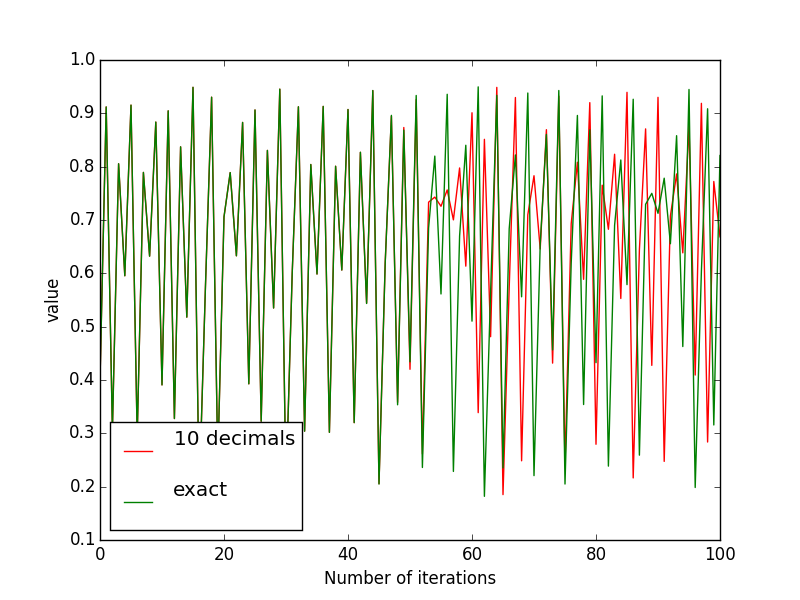
\includegraphics[width=0.5\textwidth]{dynamic_systems/logmap1}
\caption{100 Iterations of the logistic map with $a=3.8$ and $x_0 = 0.4$ computed with 10 decimals precision and exactly.}
\end{figure}
\begin{figure}\label{fig:logmapprec}
\centering
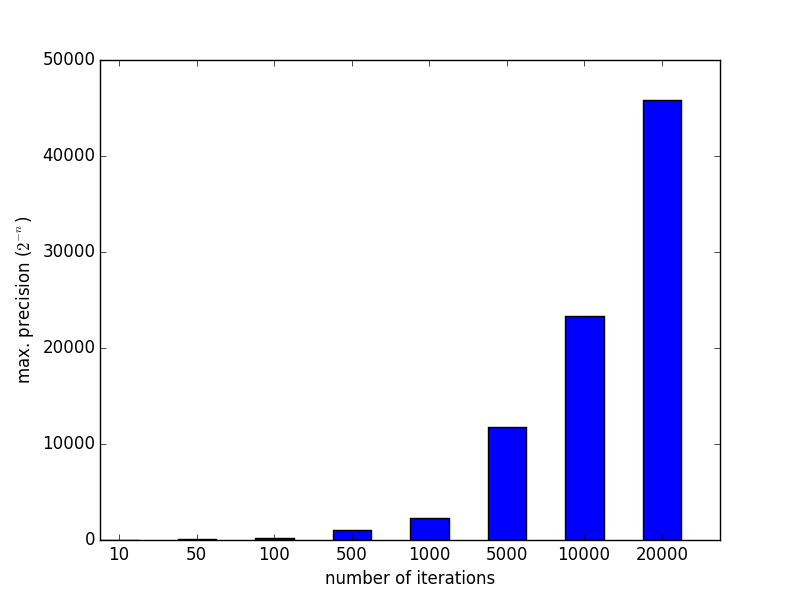
\includegraphics[width=0.5\textwidth]{dynamic_systems/logmap2}
\caption{Maximal precision iRRAM uses to compute iterations of the logistic map and output the points with 10 decimal digits.}
\end{figure}
 \subsubsection{The Shadowing Lemma}
 The term pseudo-orbit is used to describe numerically generated noisy orbits. 
 \begin{definition}\label{def:pseudoorbit}
 A sequence $(x_i)$ is called an \textbf{$\alpha$-pseudo-orbit} for a map $f$ if
 $ \| x_{i+1} - f(x_i) \| < \alpha $  
 \end{definition}
 One can think of a pseudo orbit as a numerically computed orbit, where small rounding errors can occur in every evaluation of $f$.
  \begin{definition}\label{def:shadowing}
	A real orbit $(y_i)$ \textbf{$\beta$-shadows} the pseudo-orbit $(x_i)$ if 
	$\| x_i - y_i \| < \beta$.  
 \end{definition}
 \begin{definition}
 A dynamic system is called \textbf{uniformly hyperbolic} if ...
 \end{definition}
  For systems that are uniformly hyperbolic Anosov and Bowen could show the following result \cite{anosov1967} \cite{Bowen1975} \cite{Hasselblatt:2008}:
  \begin{theorem}[Shadowing Lemma]
  For all $\beta > 0$ there exists an $\alpha > 0$ so that for every $\alpha$-pseudo-orbit $(x_i)$ there is a point $y_0$ so that the real orbit starting at $y_0$ $\beta$-shadows $(x_i)$.
  \end{theorem} 
  The logistic map is not hyperbolic...\\
  So for non-hyperbolic $f$, it can not be expected, that there is a real orbit that stays close to the pseudo orbit forever.
  Instead, there will be an orbit staying close to $(x_i)$ for some time, say up to some point $n_0$, and then starting to diverge. 
  The goal of this the case study is to investigate such orbits, in particular to find out how long there is an orbit staying close to the pseudo orbit,
  The basis for this case study is a paper by Hammel, Yorke and Grebogi from 1987 \cite{Hammel1987}.
  The paper deals with the question, how long numerical orbits of the logitstic map can be shadowed by true orbits.
  The authors show that for $a = 3.8$ and $x_0 = 0.4$, there is a true orbit $(y_n)$ of the logistic map, so that $\| x_n - y_n \| < 10^{-7}$ for $n \leq 10^7$.
  Their proof method is to compute bounds on the points of the true orbit by using a form of interval arithmetic and letting a computer do the computations. 
  All their computations are done on a Cray X-MP supercomputer. 
  For the case study, first their algorithm was implemented on a modern computer in the \cc programming language, both using fixed precision floating point numbers and \irram. 
  As a second step \irram was used to compute the shadowing orbit exactly.
    \subsubsection{The algorithm}
    The goal of the algorithm is to compute a shadowing orbit $(y_n)$ of size $N$ for a pseudo orbit $(x_n)$ of the logistic map $f$.
  Instead of computing the shadowing orbit from the first point, the algorithm computes the inverse orbit by starting with the last point and then iteratively computing the predecessor. 
  Since the logistic map is not injective, there is not a unique choice for this predecessor. 
  For some point $f(x)$ there are normally two possible values for the inverse given by $f^{-1}_{1,2}(x) = 0.5 \pm \sqrt{0.25 + \frac{x}{a}} $.
  An orbit can be computed by setting $y_N = x_N$ and then iteratively applying one of the inverse map $y_{n-1} = f^{-1}(y_n)$.   To stay close to the pseudo orbit, in every step the point on the same side of $0.5$ as $x_n$ is chosen (the index of $f^{-1}$ will from now on be omitted). 
  This works since the inverse function on $(0,1)$ is a contraction, thus
  $$ \| x_{n-1} - y_{n-1} \| = \| x_{n-1} - f^{-1}(y_n) \| \leq \| f^{-1}(x_n) - f^{-1}{y_n} \| + \| f^{-1}(x_n) - x_{n-1} \| \leq \| x_n - y_n \| + \delta $$   
  Since the original work had to do all the computations using floating point arithmetics, the inverse could not be computed exactly.
  Instead of the points $y_n$, a sequence of intervals $(I_n)$ that bound the location of $y_n$ is computed, i.e. so that $y_n \in I_n \text{ for } 0 \leq n \leq N$.
  The procedure is started with $I_N := [x_n, x_n]$ and then $I_{n-1}$ is selected so that $I_n \subseteq f(I_{n-1})$ holds and $I_n$ is chosen as small as possible. 
  Then the maximal distance between all points in $I_n$ and $x_n$ is computed.
  This gives a shadowing bound.
  \subsection{Implementation}
  The first part of the case study was to simulate the computations that were made on the Cray X-MP supercomputer on a modern computer. 
  The cray double precision data type used for the computations in the paper has machine epsilon $\varepsilon_\mu = 2^{-95}$.
  To compute the intervals $I_n$ from $I_{n+1}$ the inverse of the interval is computed as described above (using floating point arithmetic).
  Then as long as $I_{n+1} \not \subseteq f(I_n)$, $I_n$ is enlarged on both sides by the minimal possible quantity $\varepsilon_\mu$. 
  Since also the computation of $f(I_n)$ is done using floating point arithmetics, the condition might still not be fulfilled.
  This can, however, be compensated by further enlargening the interval on both sides by the constant $10^{-25}$.
  Since the precision of the clay double data type differs from the IEEE double precision, it was not possible using \cc's built in data types for simulating the algorithm.
  Instead, the boost multiprecision library \cite{boostmultiprecision} was used. 
  The library provides data types that replace the native \cc floating point types, but with a user defined precision. 
  For the interval arithmetic an interval class was implemented, having the following methods:\\
  CLASS DIAGRAM \\
  The same algorithm was also implemented in a different way. 
  Instead of using intervals with fixed precision floating point end points, \irram's \code(INTERVAL) type can be used. 
  The data type provides interval arithmetic for intervals with real numbered end points.
  Then, the inverse of an interval can be computed exactly.
  The next step, was to compute the shadowing orbit exactly.
  For that, only the pseudo orbit was calculated using floating point arithmetics. 
  Then, starting with the last point of the pseudo orbit the inverse was conputed exactly and the distance to the corresponding point in the pseudo orbit calculated.
  The maximum of all those distances is the distance of the shadow orbit and the pseudo orbit.
  One has to be a little careful though, when computing this maximum, since comparing two real numbers is not computable. 
  This problem can, however, easily be solved by the use of multi valued functions. 
  \subsection{Evaluation}
  \subsubsection{Comparison with original work}
  The original work mainly deals with the case $a=3.8$ and $x_0 = $.

  Shadowing bound for different parameters
  Breaking point for different precisions
  Real orbit?
